\documentclass{book}
\usepackage[utf8]{inputenc}
\usepackage[T1]{fontenc}
\usepackage[slovak]{babel}
\usepackage{amsmath}
\usepackage{listings}
\usepackage{graphicx}
\usepackage{epstopdf}




\lstdefinelanguage{mojMatlab}[]{Matlab} {morekeywords={mojafunkcia,mojadruhafunkcia},
sensitive=true,
alsoletter={_}
}

\begin{document}

\tableofcontents

\begin{figure}
\centering
  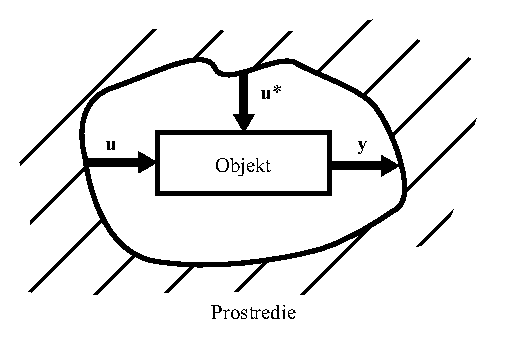
\includegraphics[width=5cm]{OBRAZOK1_1}
  \caption{Moj obrazok}
  \label{odkaznaobrazok}
\end{figure}

\chapter{Kod}

Moja funkcia \lstinline{funkcia()} je skvela.

\begin{lstlisting}[language=Matlab]
A=eig(B); %Vlastne cisla
\end{lstlisting}

\lstinputlisting[language=mojMatlab, firstline=2,lastline=2]{matlabsubor.m}






\chapter{Matika}

\begin{eqnarray}
\left[\frac{\partial f}{\partial x}\right]
\end{eqnarray}

\begin{eqnarray}
(\nabla f(x))
\end{eqnarray}

A toto je inline matematika, premenna $A$ a vzorec $x=ay+b$. A teraz pride
\begin{eqnarray}
\label{teoriarel}
E_a&=&mc^2\\
\nonumber
y&=&ax+b\\
J=\sum_{i=0}^{\infty}(a+b)\\
T=\int_{t=0}^{t=\infty}x\\
\ddot{y}+\dot{y}=0\\
\sin x = 0\\
\min_a = a^2\\
a\rightarrow b\\
\Delta_b+\delta_c=0\\
P(s)=\frac{K}{\tau s^2+1}
\end{eqnarray}

V Rov. \eqref{teoriarel} Einstein popisal... Do textu taktiez mozeme pisat $\sin x$ a taktiez $\sum a$

\begin{enumerate}
\item prvy bod
\begin{enumerate}
\item podkategoria
\item dalsia
\end{enumerate}
\item druhy bod
\item treti bod
\end{enumerate}

\chapter{Dalsia kapitola zo suboru}

Toto tahame zo suboru.

\chapter{Vlozil som kapitolu}

adnakjsnd

\chapter{Toto je kapitola}
Text kapitoly

Takto mozem aj \emph{sikmo} pisat.

Poznamku pod ciarou mozem pisat takto\footnote{Toto je moja poznamka pod ciarou}. To je dalsia poznamka pod ciarou\footnote{Blah blah blah}.

\section{Toto je podkapitola}
\label{mojapodkapitola}
Skvely text podkapitoly

\subsection{Toto je pod-podkapitola}
Dalsi skvely text

\subsubsection{Toto je pod-podpodkapitola}
Dalsi skvely text

\chapter{Dalsia kapitola}

Moje genialne myslienky

\section{Dalsia podkapitola}

Dalsia podkapitola

V Kap. \ref{mojapodkapitola} na strane \pageref{mojapodkapitola} sme pisali toto a toto a teraz 

\end{document} 